% SyncBox manual - Hardware
% Written by Christopher Thomas.
%
% Copyright (c) 2021 by Vanderbilt University. This work is released under
% the Creative Commons Attribution-ShareAlike 4.0 International License.

\chapter{Hardware}
\label{sect-hardware}

The {\projectname} was implemented as a ``shield'' that mates with a 
commercial Arduino Mega2560 r3 board. A schematic for this shield is shown 
in Figure \ref{fig-schematic}, and a layout plot in Figure \ref{fig-pcb}. 
As of January 2017, a pre-amplifier was added for the light sensor inputs;
this is indicated in simplified form in Figure \ref{fig-schematic}.

Salient features are as follows:

\begin{itemize}
\item Individual digital output signals (timing and reward) are wired to 
dedicated BNC connectors (with an additional SMB connector for the timing 
signal).

\item Joystick inputs are accepted from BNC connectors, and divided using 
pairs of 470~k$\Omega$ resistors. This maps the joystick signal range 
(0-5V) to the analog to digital converter range (0-2.56V).

\item Light sensor inputs are accepted from BNC connectors, with the 
negative terminal fed through a 10~k$\Omega$ resistor to ground. The light 
sensors are phototransistors, which behave as current sources; a 
10~k$\Omega$ resistor converts the photocurrent to a voltage large enough 
to measure reliably but small enough to leave ample headroom for device 
and light source variation.

The pre-amplifier has a gain of 10x, and performs high-pass filtering with
a time constant of several seconds to cancel DC bias. The system should be
allowed to stabilize for one minute after being connected and powered,
prior to use.

\item The NeuraLynx handshaking signals are implemented using two 
dedicated ATmega output ports, for speed of manipulation by firmware. 
The ports chosen each map to contiguous blocks of 8 pins on the Arduino 
Mega header, which are wired to an appropriate 34-pin connector.

In 16-bit mode, bit 15 is the strobe bit, and bits 0-14 are data.

In 8-bit mode, bit 15 is still the strobe bit, bits 8-14 are data, and 
bits 0-7 are always zero. \textbf{NOTE:} The user sees this as an 8-bit 
interface. The argument to ``NEU'' is 0-127.

\item A status LED is provided, to communicate diagnostic information. 
This is not presently used (it's turned on when the {\projectname} boots 
and is left on).

\item A reset switch is provided, for manual reset without power cycling. 
In practice, power cycling is likely the most convenient reset method.

\item All traces and cables are assumed to be ``electrically short'' -- 
that is, to have propagation delays very much smaller than the timescales 
relevant to the equipment being connected. This allows cable termination 
and driving impedence to be ignored.

A rule of thumb is that reflections propagate at a minimum of half the 
speed of light, and that ten round-trips is sufficient to stabilize signal 
levels. With a characteristic timescale of 0.1~ms, maximum cable length is 
about 750~m.

If connected equipment uses a sufficiently fast communications sampling
rate (50 MHz or more), reflections may become significant.
\end{itemize}

A reverse-engineered schematic of the joystick is shown in Figure 
\ref{fig-joystick}.

\begin{figure}[p]
\begin{center}
\includegraphics[height=0.4\textheight]{schematics/synchbox-shield-schem.png}
\end{center}
\caption{{\projectname} schematic.}\label{fig-schematic}
\end{figure}

\begin{figure}[p]
\begin{center}
\includegraphics[height=0.4\textheight]{schematics/joystick-2016-schem.png}
\end{center}
\caption{Joystick schematic.}\label{fig-joystick}
\end{figure}

\begin{figure}[p]
\begin{center}
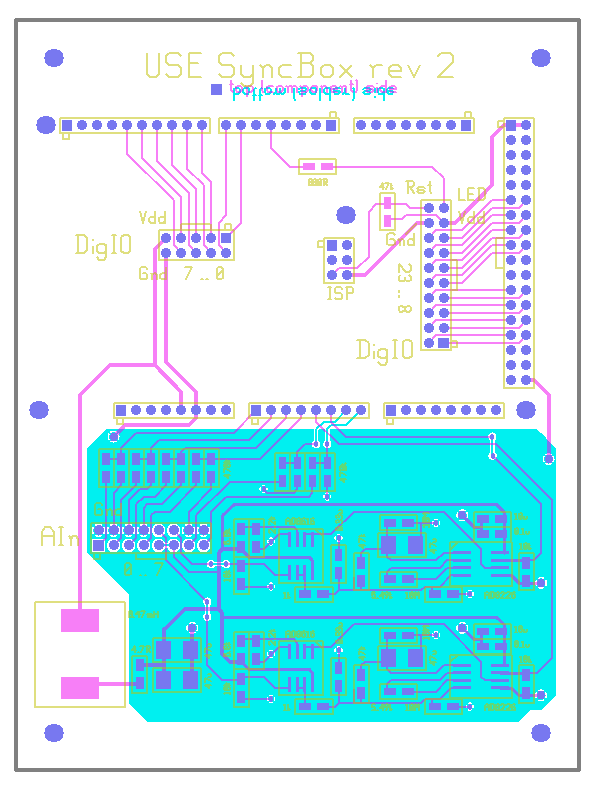
\includegraphics[height=0.9\textheight]{layouts/synchbox-shield-layout.png}
\end{center}
\caption{{\projectname} PCB layout.}\label{fig-pcb}
\end{figure}

%
% This is the end of the file.
